\chapter{Partitioned Priors}

One way in which we may try to improve the performance of local, single-site, Metropolis-Hastings is by paritioning the prior distribution into several component parts. The idea behind this approach is that we may be able to guide the resampling process as to improve the convergence to the mode and the mixing properties of simple Metropolis-Hastings. \todo{say something about proposal kernels vs. sampling from prior?}

Based on this idea, it may be possible to design a light pre-inference rewriting of a probabilistic program which splits up its priors so that the subsequent inference step is performed more efficiently.

In this chapter we focus on the splitting of uniform continuous priors. Not only are such priors commonly used in models, but sampling from any distribution ultimately relies on uniformly drawn random bits. Speeding up inference on uniform priors may therefore lead to speed ups on other distributions, assuming certain desirable properties, such that small changes in the uniform bits correspond to small changes in the final distribution. \todo{not sure if this makes much sense. Need to research it more or remove}

For simplicity, we also focus on models with a uni-modal posterior distribution. The analysis for multi-modal distributions would follow similar lines to the one presented here, but would also have to additionally account for mode-switching. We will look closer at this problem in Chapter \ref{whoKnows}.

\section{Preliminaries}

In order to explore the partitioned prior idea we need to have an understanding of the basic Metropolis-Hastings algorithm. We also need a way to evaluate the performance of a certain partition, which we propose to do by looking separately at the time it takes for our Markov Chain to reach the true posterior's mode and at the chain's mixing properties around this mode.

\subsection{Local Metropolis-Hastings}
\todo{add basic explanation}

\subsection{Expected number of iterations to a neighbourhood of the mode}
\label{section:sampsToMode}
The first test of the efficiency of a partition which we propose is, on average, how many iterations the algorithm will have to go through before the markov chain reaches a state close to the mode of the posterior. Since we are interested in seeing our markov chain mix around the posterior's mode, we want it to get close to the mode as soon as possible. The average number of iterations to the mode can also be viewed as a way to estimate a lower bound on the burn-in we should set for our algorithm.

When using local Metropolis-Hastings with an unpartitioned uniform prior, it is easy to analytically calculate the expected number of iterations to a mode's neifghbourhood. Using the unpartitioned prior (uniform-continuous a b), we end up sampling from the uniform distribution and accepting or rejecting those samples according to the Metroplis-Hastings acceptance ratio. In order to reach some neighbourhood of the mode $[mode - \epsilon, mode + \epsilon]$, we need to actually sample a number in that range from the prior (sample which will definitely be accepted since it will have higher log likelihood than anything outside that range). This means the number of samples it will take to get close to the mode with an unpartitioned prior will follow a geometric distribution with $p = (2\epsilon)/(b-a)$. The expected number of samples it takes to reach the neighbourhood will then be $(b-a)/(2\epsilon)$.

For partitioned priors it will usually not be possible to analytically determine the expected number of steps to $[mode - \epsilon, mode + \epsilon]$, so we shall instead make use of empirical tests.

\subsection{Mixing properties around the mode}
Once the markov chain has reached the mode we will wish to see how well it manages to mix around it. Here we will look at different metrics that might give us an idea of the mixing properties. Visually inspecting the sample evolution will show if the inference tends to get stuck on certain values for longs stretch. A numerical estimate of this can be obtained by measuring the ``distance'' traveled by the merkov chain around the mode (i.e. the sum of absolute differences between consecutive samples). We can also inspect the sample autocorrelation, with the idea that good mixing properties should imply a small autocorrelation within a sample run.

\section{Sum of uniforms}

We first consider partitioning the uniform prior into a sum of uniforms. This choice is made for simplicity and in order to observe some basic properties concerning local Metropolis-Hasting's performance on partitioned priors.

Such a partitioning, however, should not be used in actual probabilistic program compilation techniques since it does not leave the prior invariant (that is to say, a sum of uniform variables is not a uniform variable, see Figure \ref{fig:1295Prior}). The invariance is due to the uniform distribution not being infinitely divisible. The approach presented here could be safely used on other distributions, such as Gammas and Gaussians, which are infinitely divisible. In Section \ref{next} we will present a partitioning technique which does leave the uniform prior unchanged.

\begin{figure}[H]
    \centering
    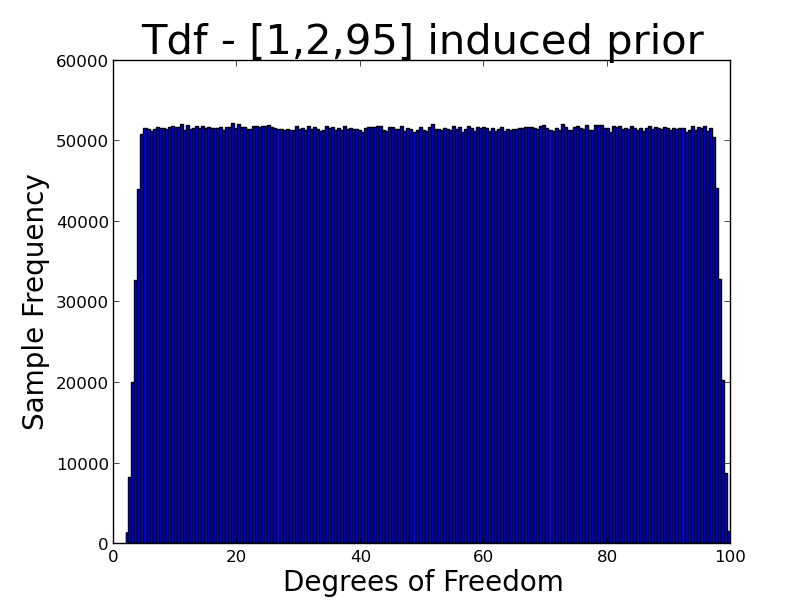
\includegraphics[width=0.8\textwidth]{Tdf1295Prior.png}
    \caption{Prior distribution induced by partitioning the prior (uniform-continuous 2 100) into (uniform-continuous 2 95) + (uniform-continuous 0 2) (uniform-continuous 0 1).}
    \label{fig:1295Prior}
\end{figure}

\subsection{Finding a good sum decomposition}

First we look at the expected number of steps needed to reach a neighbourhood of the mode. As explained in Section \ref{section:sampsToMode}, the expected number of steps to $[mode - \epsilon, mode + \epsilon]$ of the mode can be analytically computed for the unpartitioned prior (uniform-continuous a b) as being $(b-a)/(2\epsilon)$.

For the partitioned priors, we instead perform empirical tests. These tests measure how many samples it takes for different partitions to reach neighbourhoods of the mode of different sizes. One thousand runs are done for each partition and neighbourhoods of 0.5, 0.25, 0.1 and 0.01 are considered. The partitions consited of between 2 and 5 values which were drawn with replacement from [0, 0.5, 1, 2, 5, 7, 10, 15, 20, 25, 30, 35, 40, 45]. A final component value is added such that the sum of all components is the uniform prior specified in the Tdf model, namely (uniform-continuous 2 100). We specify partitions in the format (x,y,z) meaning (uniform-continuous 0 x) + (uniform-continuous 0 y) + (uniform-continuous 2 z). All considered partitions respect the constraint $x+y+z = 98$.

Table \ref{tab:bestParts} contains the empirical performance for the unpartitioned prior and for the best 2 partitions on each neighbourhood size.

\begin{table}[H]
  \centering
  \begin{tabular}{lllll}
    \toprule
    \multirow{2}{*}{Partition} & \multicolumn{4}{l}{Target neighbourhood size} \\
    \cmidrule(r){2-5} 
    & 1 & 0.5 & 0.2 & 0.02 \\
    \midrule
    Unpartitioned & 98.38 & 199.29 & 494.87 & 4919.75 \\
    (5, 93) & 89.03 & 122.87 & 172.9  & 670.14 \\
    (20, 78)& 92.55 & 142.6  & 259.21 & 1834.18 \\
    (2, 96) & 92.56 & 117.35 & 157.83 & 371.9 \\
    (1, 45, 52) & 123.97 & 146 & 172.78 & 400.01 \\
    (0.5, 2, 95.5) & 134.24 & 162.03 & 201.57 & 297.79 \\
    (1, 2, 95) & 130.06 & 155.48  & 186.83 & 317.31 \\
    \bottomrule
  \end{tabular}
  \caption{Expected number of steps to neighbourhoods of the mode on the Tdf continuous model for an unpartitioned prior and some of the best sum decomposition priors.}
  \label{tab:bestParts}
\end{table}

The best partition seems to depend somewhat on the size of the neighbourhood, but there also seem to be partitions that consistently and significantly outperform the unpartitioned prior on all the neighbourhood sizes looked at above. In fact, for epsilon values of 0.1 and 0.01 the unpartitioned prior performs worse than any of the partitioned variants. 

It also seems that, as epsilon gets smaller, it’s useful to have smaller partition components, such that we get the 0.5 partition in the best solution for a mode neighbourhood of size 0.02, while this partition size makes no appearance in the top partition lists for other neighbourhood sizes.

The second aspect of convergence that a partition might help with is the mixing rate around the mode. In order to test the priors' mixing properties we can consider what happens after the markov chain reaches the mode. Specifically, we set the initial sample to the mode of the true posterior distribution and check how much the chain moves over the next 1000 samples. Repeating this test 100 times and averaging the sum of jumps gives us the results in Table \ref{tab:partMix}.

The format is (partitions, average distance travelled, variance)

\begin{table}[H]
  \centering
  \begin{tabular}{lll}
    \toprule
    Partition & Mean distance travelled & Variance in distance travelled \\
    \midrule
    Unpartitioned & 7.75 & 13.43 \\
    (1, 1, 1, 95) & 137.55 & 393.96 \\
    (1, 1, 1, 1, 94) & 135.08 & 616.41 \\
    (1, 1, 2, 94) & 131.19 & 539.03 \\
    (1, 1, 1, 2, 93) & 129.91 & 583.16 \\
    (0.5, 1, 1, 1, 94.5) & 126.76 & 382.09 \\
    (1, 2, 95) & 125.67 & 408.16 \\
    (1, 1, 96) & 125.44 & 311.76 \\
    (0.5, 1, 2, 94.5) & 123.38 & 487.26 \\
    (1, 1, 2, 2, 92) & 122.9 & 615.54 \\
    (2, 2, 94) & 121.25 & 844 \\
    \bottomrule
  \end{tabular}
  \caption{Average distance travelled around the mode on the Tdf continuous model for an unpartitioned prior and some of the best sum decomposition priors.}
  \label{tab:bestParts}
\end{table}

This test only measures the average distance travelled (i.e. sum of absolute differences between consecutive samples), which could be a misleading measure of mixing. The large difference between the unpartitioned and the partitioned variants do suggest that there is some improvement here though. The mixing reate is investigates more thoroughly in Section \ref{next}

Based on the above results, we decide to further investigate the performance of the (1, 2, 95) partitioned prior, since this decomposition performs well both in reaching the mode and in mixing around it.

\subsection{Evaluating the (1,2,95) sum decomposition}

Table \ref{tab:bestParts} makes clear the increased speed in reaching a neighbourhood of the mode offered by the decompositions. The potential benefit conferred in mixing rate is less clear however. To test this we look at the sample evolution and autocorrelation plots for two runs obtained with an unpartitioned and a (1,2,95) partitioned prior.

\begin{figure}[H]
    \centering
    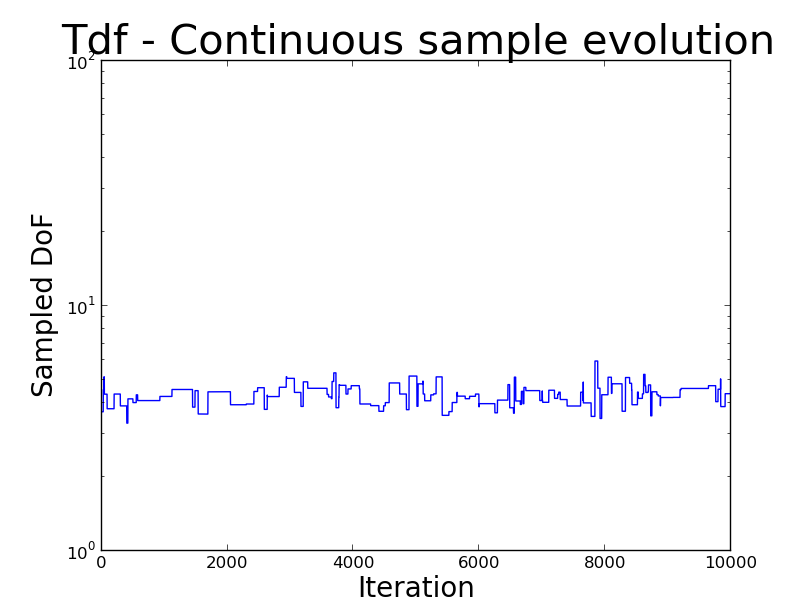
\includegraphics[width=0.8\textwidth]{TdfSampEvol.png}
    \caption{The sample evolution, over 10,000 samples, for the unpartitioned prior.}
    \label{fig:UnpSampEvol}
\end{figure}

\begin{figure}[H]
    \centering
    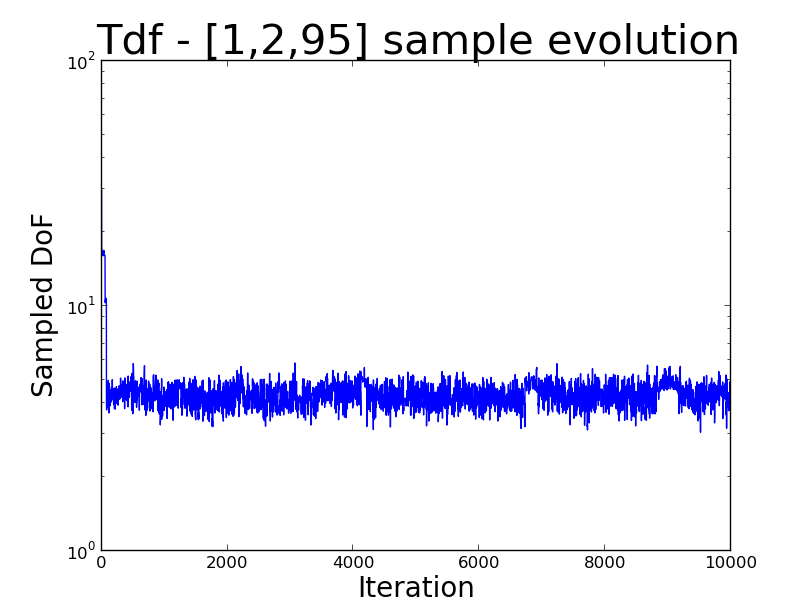
\includegraphics[width=0.8\textwidth]{Tdf1295SampEvol.png}
    \caption{The sample evolution, over 10,000 samples, for the (1, 2, 95) partitioned prior.}
    \label{fig:1295SampEvol}
\end{figure}

\begin{figure}[H]
    \centering
    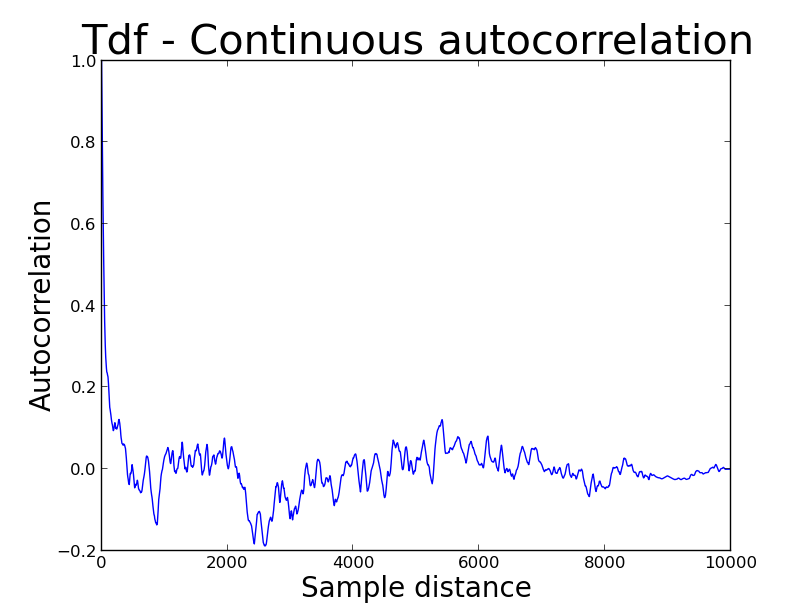
\includegraphics[width=0.8\textwidth]{TdfAutoCorr.png}
    \caption{The autocorrelation, over 10,000 samples, for the unpartitioned prior.}
    \label{fig:UnpAutoCorr}
\end{figure}

\begin{figure}[H]
    \centering
    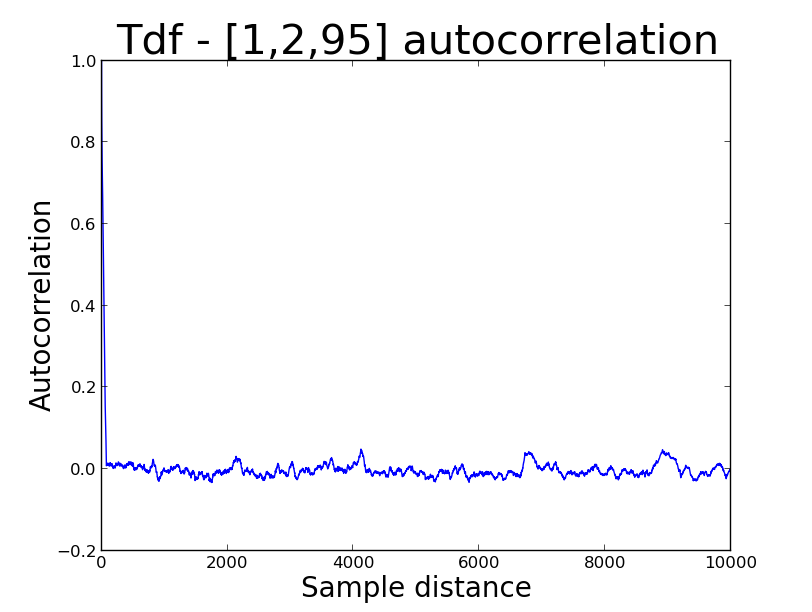
\includegraphics[width=0.8\textwidth]{Tdf1295AutoCorr.png}
    \caption{The autocorrelation, over 10,000 samples, for the (1, 2, 95) partitioned prior.}
    \label{fig:1295AutoCorr}
\end{figure}

These graphs confirm our preliminary results from Section \ref{past}, and show that the partitioned prior does help with mixing around the mode and with eliminating large correlations between consecutive samples.

The final test in determining the quality of the decomposition is to look at the actual sample distributions obtained under the two different prior formulations.

\begin{figure}[H]
    \centering
    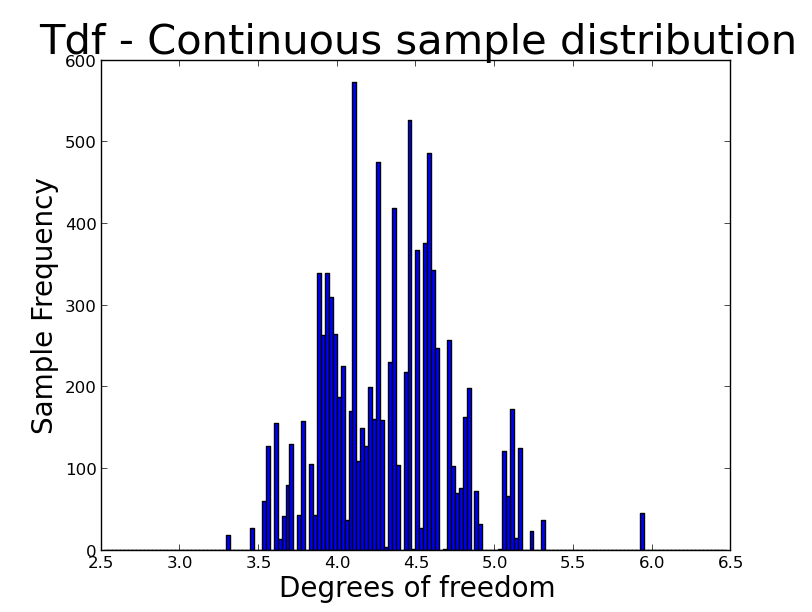
\includegraphics[width=0.8\textwidth]{TdfSampDist.png}
    \caption{The sample distribution obtained from 10,000 samples using an unpartitioned prior.}
    \label{fig:UnpSampDist}
\end{figure}

\begin{figure}[H]
    \centering
    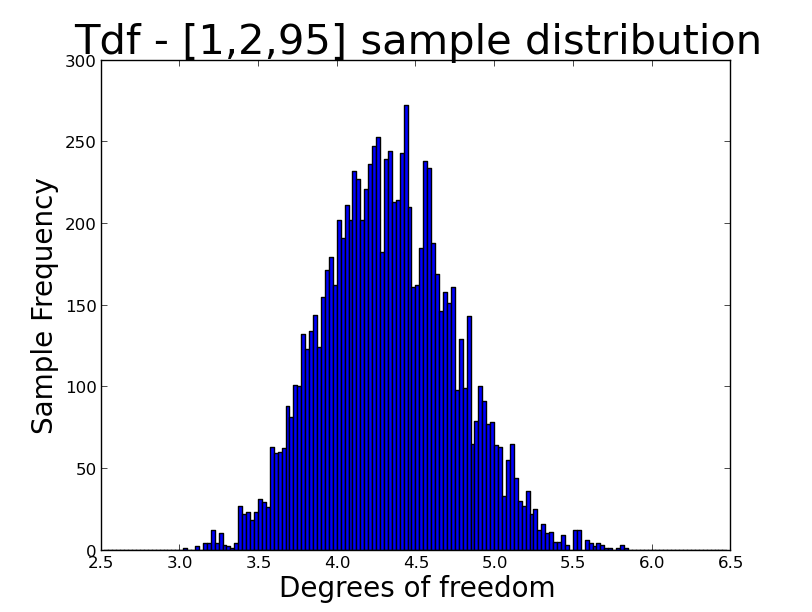
\includegraphics[width=0.8\textwidth]{Tdf1295SampDist.png}
    \caption{The sample distribution obtained from 10,000 samples using an (1, 2, 95) partitioned prior.}
    \label{fig:1295SampDist}
\end{figure}

The true posterior for the Tdf continuous model was given in Section \ref{blah}. Looking at these it is quite clear the partitioned prior outperforms the origina, unpartitioned, variant. However, this result may be misleading since we are evaluating it on the same distribution which we used to choose the form of the partition. To test the robustness of our partition we repeat the above tests on a new model.

\subsubsection{The Tdf21 model}
In order to test our decomposition on a different posterior distribution, we generate 1,000 datapoints from a Student t distribution with 21 degrees of freedom and condition the Tdf Continuous model on this new dataset. The resulting posterior is shown in Figure \ref{fig:21Post}.

\begin{figure}[H]
    \centering
    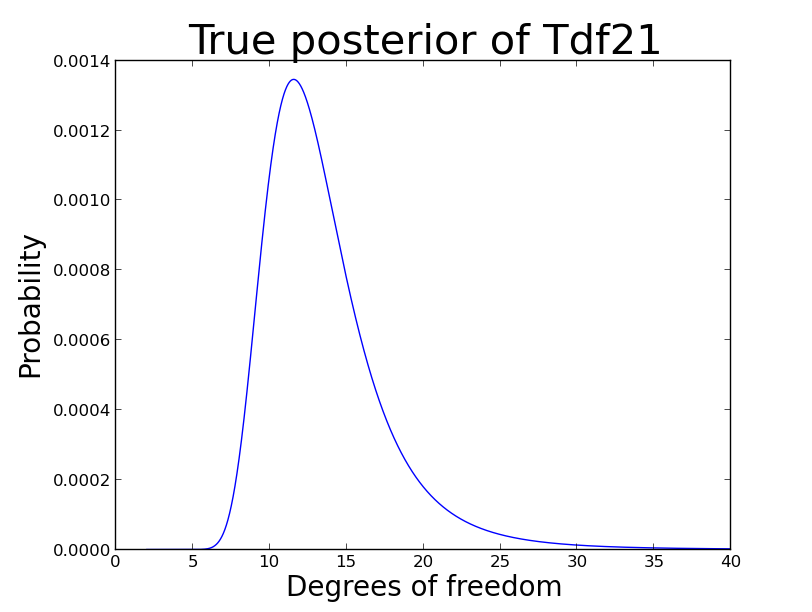
\includegraphics[width=0.8\textwidth]{Tdf21Post.png}
    \caption{The true posterior of the Tdf21 model}
    \label{fig:21Post}
\end{figure}

The mode here is actually 11.5. This is probably due to the fact that 1000 datapoints are not enough to accurately pinpoint a student-t with so many degrees of freedom (21) since, as the number of degrees of freedom increases, the differences between corresponding student-t distributions shrinks. 
The posterior distribution is however significantly different from the one for the previous dataset, which should be sufficient for testing the properties of the priors.

In order to better understand how the Metropolis-Hastings algorithm will be affected by this change we can also look at the log-likelihoods induced by the original Tdf Continuous model and by the Tdf21 model.

\begin{figure}[H]
    \centering
    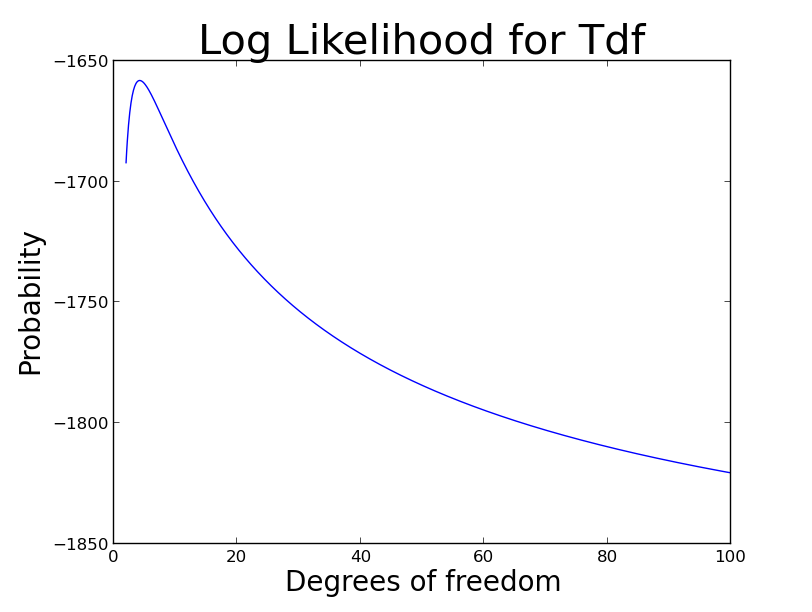
\includegraphics[width=0.8\textwidth]{TdfContLL.png}
    \caption{The log-likelihood of the Tdf Continuous model.}
    \label{fig:TdfLL}
\end{figure}

\begin{figure}[H]
    \centering
    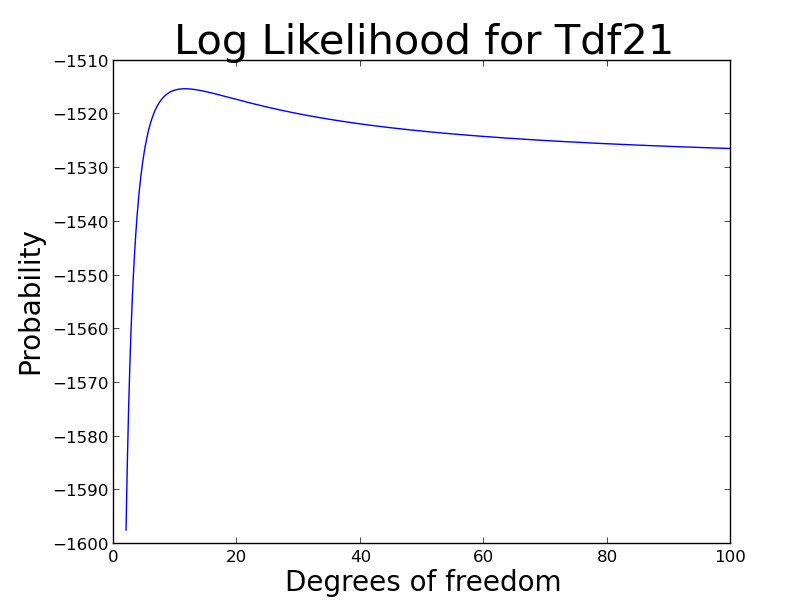
\includegraphics[width=0.8\textwidth]{Tdf21LL.png}
    \caption{The log-likelihood of the Tdf21 model.}
    \label{fig:Tdf21LL}
\end{figure}

As can be seen, the Tdf21 log-likelihood is much flatter than the one for the original model. By repeating the mixing tests performed above we can test the effect of this difference.

\subsubsection{Evaluating the decomposition on the Tdf21 model}
On this new model posterior we can now test the convergence of the priors by once again plotting the sample evolution, the sample autocorrelation and the sample distributions. The partitioned prior is the same one we used on the previous datapoints, namely (1,2,95)

\begin{figure}[H]
    \centering
    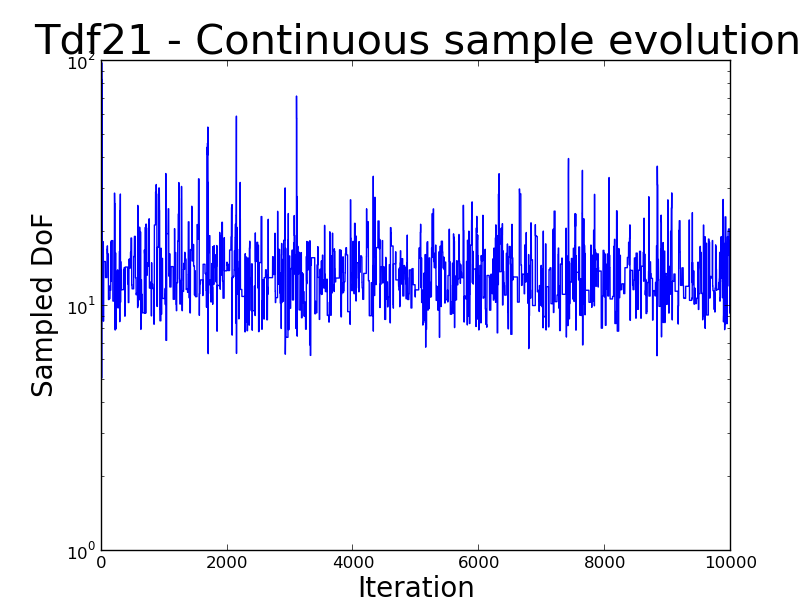
\includegraphics[width=0.8\textwidth]{Tdf21SampEvol.png}
    \caption{The sample evolution, on the Tdf21 model for, the unpartitioned prior.}
    \label{fig:21UnpSampEvol}
\end{figure}

\begin{figure}[H]
    \centering
    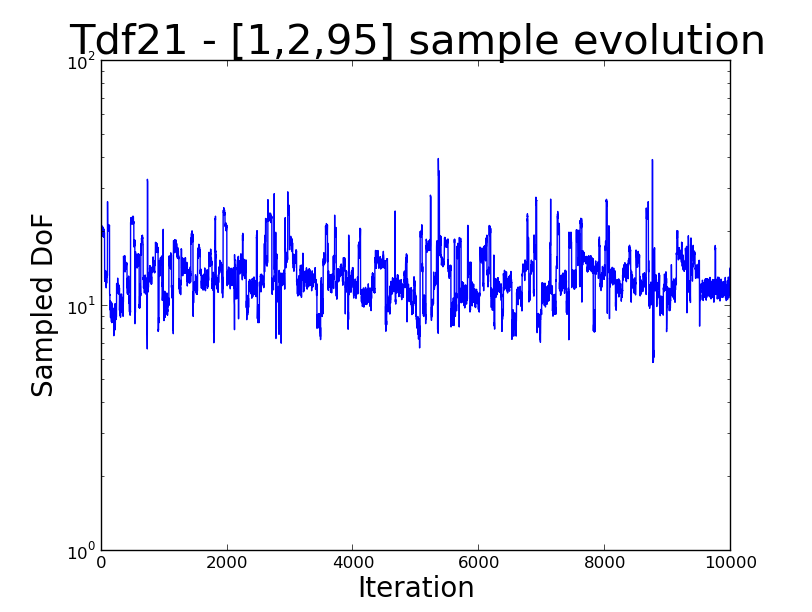
\includegraphics[width=0.8\textwidth]{Tdf211295SampEvol.png}
    \caption{The sample evolution, on the Tdf21 model for, for the (1, 2, 95) partitioned prior.}
    \label{fig:211295SampEvol}
\end{figure}

From the sample evolutions we can see that the partitioned samples tend to clump a little more since bigger changes in the samples only occur when the 95 component changes. Both versions seem to mix well though.

\begin{figure}[H]
    \centering
    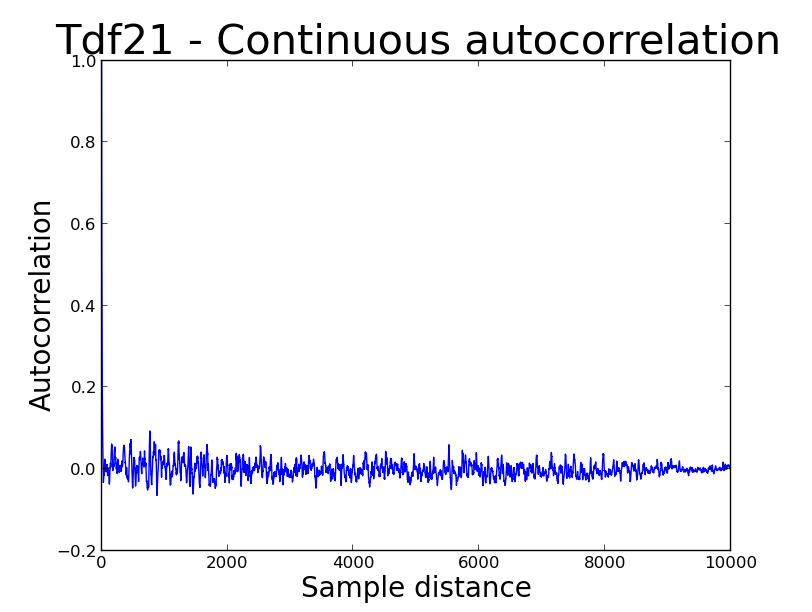
\includegraphics[width=0.8\textwidth]{Tdf21AutoCorr.png}
    \caption{The autocorrelation, on the Tdf21 model for, for the unpartitioned prior.}
    \label{fig:21UnpAutoCorr}
\end{figure}

\begin{figure}[H]
    \centering
    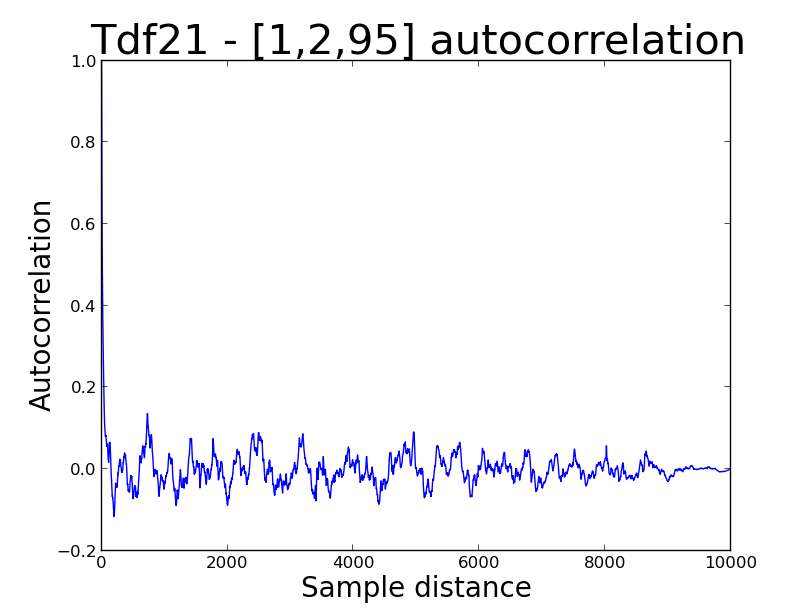
\includegraphics[width=0.8\textwidth]{Tdf211295AutoCorr.png}
    \caption{The autocorrelation, on the Tdf21 model for, for the (1, 2, 95) partitioned prior.}
    \label{fig:211295AutoCorr}
\end{figure}

The autocorrelation plots are also more similar than in the case of the original Tdf model. The unpartitioned prior does quite well here since the flat shape of the log-likelihood means there is a higher chance that a proposition drawn from the prior will be accepted by the Metropolis-Hastings algorithm.

The final test has to again be the actual sample distributions.

\begin{figure}[H]
    \centering
    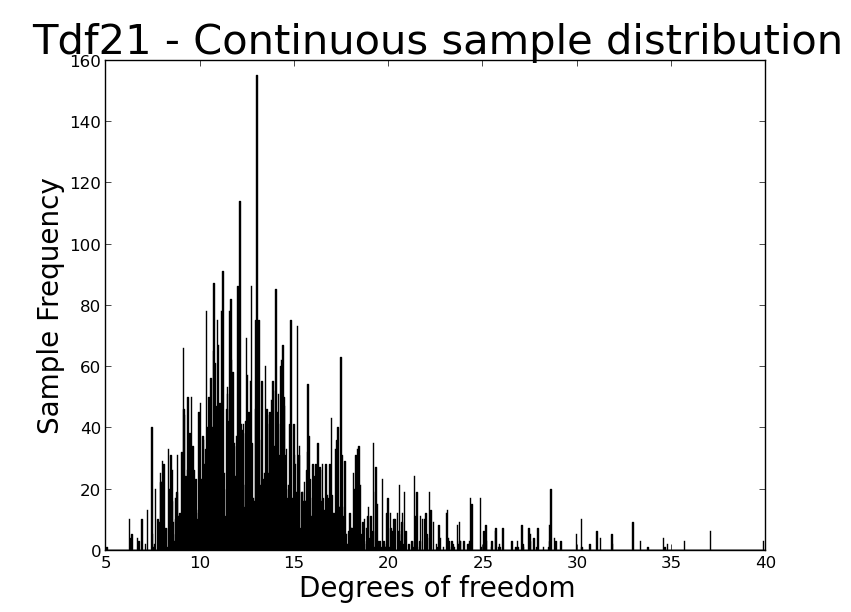
\includegraphics[width=0.8\textwidth]{Tdf21SampDist.png}
    \caption{The sample distribution obtained from 10,000 samples using an unpartitioned prior on the Tdf21 model.}
    \label{fig:21UnpSampDist}
\end{figure}

\begin{figure}[H]
    \centering
    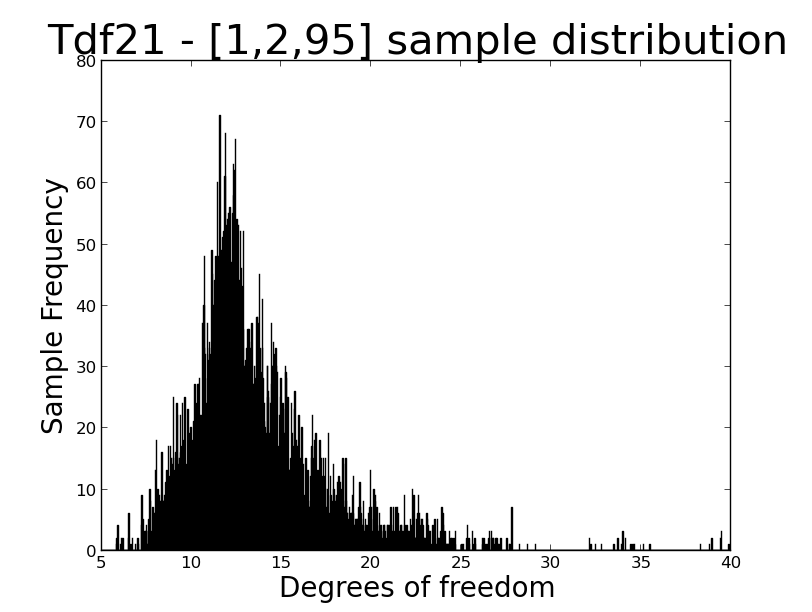
\includegraphics[width=0.8\textwidth]{Tdf211295SampDist.png}
    \caption{The sample distribution obtained from 10,000 samples using an (1, 2, 95) partitioned prior on the Tdf21 model.}
    \label{fig:211295SampDist}
\end{figure}

Here we can see that the partitioned prior still results in a smoother distribution that does a better job of representing the true posterior.

\section{Bit decomposition}
As mentioned in Section \ref{blah}, one problem with the sum of uniforms decomposition is that it alters the shape of the prior. We would like to come up with decompositions that leave the prior invariant so that, since such decompositions could be applied indescriminately to re-write any probabilistic program. A family of invariant partitions of an uniform prior can be constructed by considering the bit representation of the uniform samples up to a certain depth and then adding a single uniform-continuous value of the correct size.

\subsection{Definition}
In order to partition any uniform interval (uniform-continuous a b) it is sufficient to be able to partition the interval (uniform-continuous 0 1). Once this is accomplished, the target interval can be obtained as (uniform-continuous a b) = a + (b-a) * (partitioned(uniform-continuous 0 1)).

In order to partition the interval (uniform-continuous 0 1) we first pick a bit depth, k, we wish to partition to such that $ k \in \{ 0, 1, \ldots \infty \} $ We then define (uniform-continuous 0 1) $= flip*2^{-1} + flip*2^{-2} \ldots + flip*2^{-k} +$ (uniform-continuous 0 $2^{-k}$), where flip is a function which flips a coin and return 0 or 1 with probability 1/2 each.

\subsection{Evaluation on Tdf and Tdf21}

To get an idea of the properties of this decomposition we perform an empirical evaluation on the Tdf continuous model and on the Tdf21 model.

Looking at mixing rates \ref{fig} shows that a 3rd degree bit decomposition obtains similar performance to the unpartitioned prior. Intuitively this is because we are still subjecting proposals to the Metropolis-Hastings acceptance ratio, so if our program decides to flip one of the leading bits the proposal will be rejected, leading to bad mixing. As the depth of the bit decomposition increases, however, the smaller the probability that one of the leading bits are picked and therefore the better we will expect the mixing to be. \todo{Should be possible to give some more formal results here.} We, however, restrict ourselves to a 3rd degree decomposition here since a higher degree variant would exhibit other problems, which are discussed in Section \ref{dd}.

\begin{figure}[H]
    \centering
    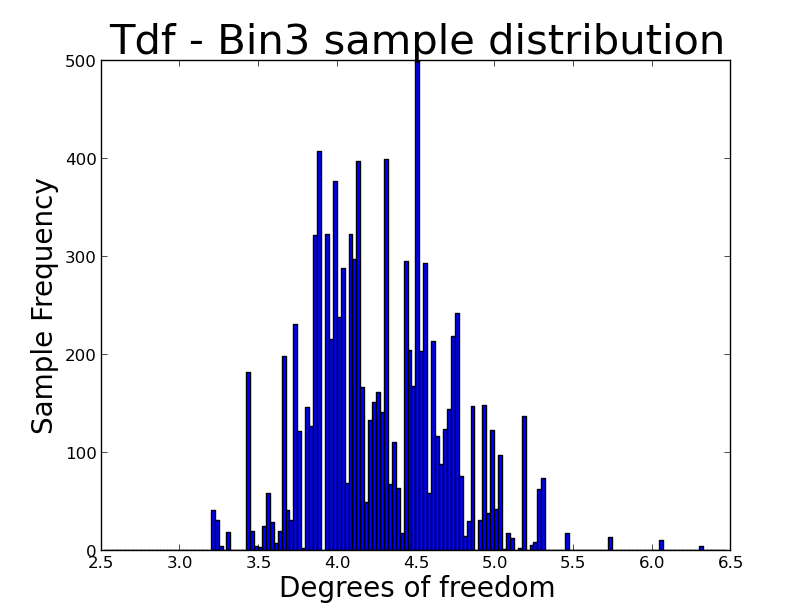
\includegraphics[width=0.8\textwidth]{TdfBin3SampDist.png}
    \caption{The sample distribution obtained from 10,000 samples using a 3rd degree bit decomposition on the Tdf model.}
    \label{fig:B3SampDist}
\end{figure}

\begin{figure}[H]
    \centering
    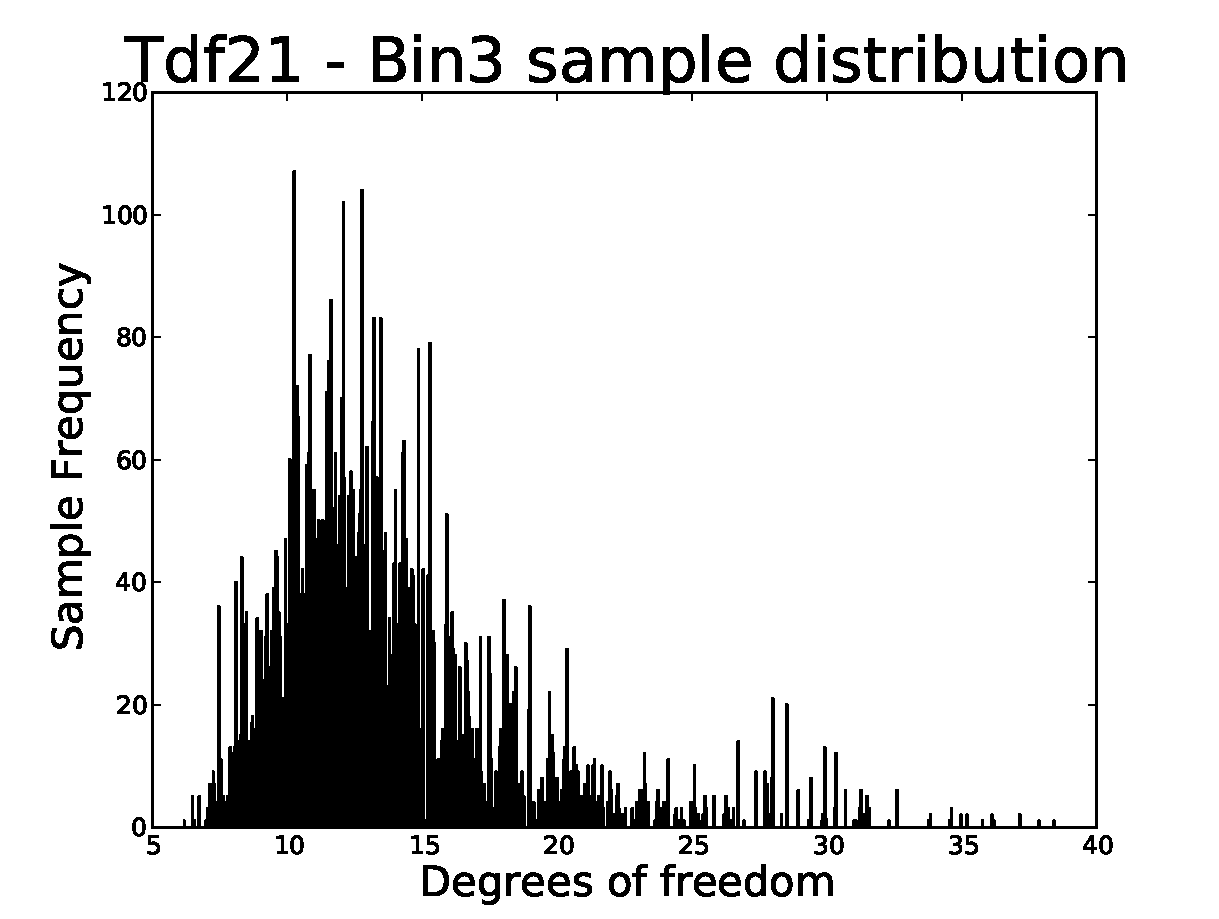
\includegraphics[width=0.8\textwidth]{Tdf21Bin3SampDist.png}
    \caption{The sample distribution obtained from 10,000 samples using a 3rd degree bit decomposition on the Tdf21 model.}
    \label{fig:21B3SampDist}
\end{figure}

Turning to the expected time to reach (see Table \ref{tab}) the mode reveals that the 3rd degree binomial provides a significant improvement on the unpartitioned prior, though not as significant as the sum of uniforms does. \todo{talk about how binomials of different depth perform here}


